%!TEX root = ../thesis.tex

\section{ソフトウェアの設計}
AI-Formulaで使用される屋外自律高速モビリティを対象として経路追従ソフトウェアの開発を行う.
AI-Formulaで使用するモビリティには複数のセンサが搭載されているが, ここで経路追従に用いることができるセンサはステレオカメラかGNSS+IMUセンサが挙げられる.
AI-Formulaのコンテスト会場となるAIモビリティパーク紫峰は周囲に高い建造物の無い立地であるため, GNSSのマルチパスの影響が少ないと考えられる.
そのため, 本研究ではGNSSに基づいた経路追従ソフトウェアの開発を行う.

% \begin{figure}[H]
%   \centering
%  \includegraphics[keepaspectratio, scale=0.2]
%       {images/system.png}
%  \caption{Path following system}
%  \label{fig:system}
% \end{figure}

GNSSを用いて経路追従を行うためには, 位置に加えて方向のデータも必要となる.
モビリティに搭載されているGNSS+IMU(VectorNav VN-200)は方位も計測できる仕様であるため, 方向のデータの取得にもVN-200を使用する.
GNSS+IMU(VectorNav VN-200)はvectornav\cite{vectornav}というROS 2ラッパのパッケージが公開されているため, 本研究ではそれを使用する.
%
%
自律走行では, 目標経路の座標とGNSSから得たデータの座標を利用してPure pursuitによる経路追従を行う.
Pure pursuitはFig.4.1に示すように, 目標経路上において自己位置より前の位置に逐次的に目標地点を定め, 目標地点に追従していく手法である.
モビリティが移動するにつれて目標地点も更新されるため, 結果として目標結果に沿った追従動作を行う.
% 
\begin{figure}[H]
  \centering
 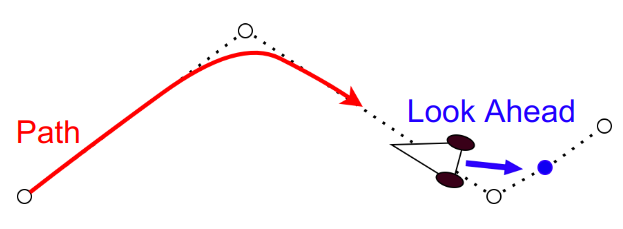
\includegraphics[keepaspectratio, scale=0.5]
      {images/PurePursuit.png}
 \caption{Pure pursuit algorithm}
 \label{fig:system}
\end{figure}
% % 
目標地点との角度差を取得し, その角度差に対してPID制御を行うことでモビリティの角速度を決定する.
並進速度は一定として, 求めた角速度に基づいてモビリティを制御する.
Fig.4.2に開発するソフトウェアの構成を示す.

\begin{figure}[H]
     \centering
    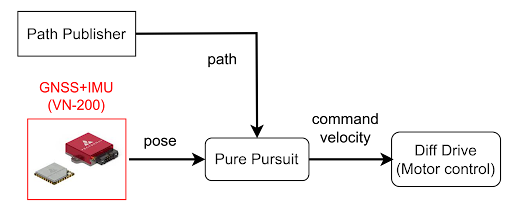
\includegraphics[keepaspectratio, scale=0.6]
         {images/SimpleSystem.png}
    \caption{Path following system}
    \label{fig:system}
\end{figure}

\section{目標経路の作成}
経路追従をする際には追従するための目標経路が必要となる.
作成した経路追従のソフトウェアは, 事前にシミュレータ環境や手動走行をさせた時にGNSSから得た座標データをCSVファイルに経路情報としてまとめている.
% 
CSVファイルにまとめられた経路情報は測地座標系のデータであり, UTM座標系に変換して目標経路として使用する.
GNSSから得たデータはECEF座標系で取得されるため, 目標経路の座標系と合わせるためにUTM座標系に変換する.
% 
UTM座標系に変換されたデータに対し, 3次スプライン補間を適用することで, 滑らかで連続性のある目標経路を作成する.
% 
% UTM座標系に合わされた目標経路の座標と自己位置の座標を利用してPurePursuitによる経路追従を行う
% 
Fig.4.3に目標経路の作成手順を示す.
Fig.4.4に作成した目標経路の例を示す.
ここで, 示した目標経路は走行時に取得したGNSSデータをGoogleMap上でプロットしたものである.

\begin{figure}[H]
     \centering
    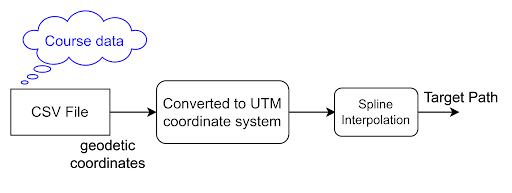
\includegraphics[keepaspectratio, scale=0.6]
         {images/navigationData.png}
    \caption{Target path system}
    \label{fig:target path}
\end{figure}

\begin{figure}[H]
  \centering
 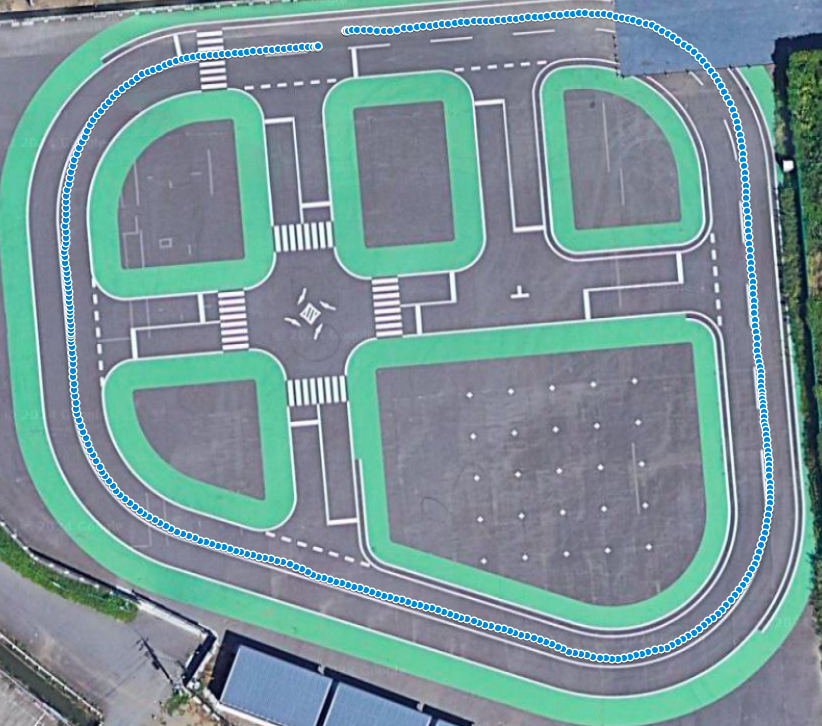
\includegraphics[keepaspectratio, scale=0.3]
      {images/targetpath.png}
 \caption{Predefined target trajectory}
 \label{fig:target path}
\end{figure}


\newpage